\documentclass[11pt]{article}
\usepackage[a4paper,margin=1in]{geometry}
\usepackage{graphicx,booktabs,amsmath,xcolor,microtype}
\usepackage{tikz}\usetikzlibrary{positioning,arrows.meta,calc,fit,backgrounds,decorations.pathreplacing,shapes.geometric}
\usepackage{caption}\usepackage{enumitem}\usepackage{placeins}\usepackage{listings}\usepackage{float}\usepackage{needspace}
\renewcommand{\topfraction}{0.94}\renewcommand{\bottomfraction}{0.9}
\renewcommand{\textfraction}{0.06}\renewcommand{\floatpagefraction}{0.8}\setcounter{topnumber}{4}\setcounter{totalnumber}{5}
\usepackage[hidelinks]{hyperref}
\definecolor{ink}{HTML}{16324F}\definecolor{accent}{HTML}{B5172F}\definecolor{green}{HTML}{1B7837}
\definecolor{amber}{HTML}{C77D11}
\definecolor{lightink}{HTML}{E8EEF4}\definecolor{lightaccent}{HTML}{F6E2E5}\definecolor{lightgreen}{HTML}{E2F0E6}
\definecolor{lightamber}{HTML}{F7ECD9}\definecolor{grey}{HTML}{7A7A7A}
\captionsetup{font=small,labelfont=bf,labelsep=period}
\renewcommand{\arraystretch}{1.25}
\setlist{leftmargin=1.4em,itemsep=2pt,topsep=3pt}
\tikzset{
  box/.style={draw=ink,fill=lightink,rounded corners=2pt,inner sep=6pt,align=center,font=\small},
  redbox/.style={draw=accent,fill=lightaccent,rounded corners=2pt,inner sep=6pt,align=center,font=\small},
  greenbox/.style={draw=green,fill=lightgreen,rounded corners=2pt,inner sep=6pt,align=center,font=\small},
  amberbox/.style={draw=amber,fill=lightamber,rounded corners=2pt,inner sep=6pt,align=center,font=\small},
  plain/.style={align=center,font=\small},
  flow/.style={-{Latex[length=2.2mm]},draw=ink,thick},
  redflow/.style={-{Latex[length=2.2mm]},draw=accent,thick},
  greenflow/.style={-{Latex[length=2.2mm]},draw=green,thick},
  lbl/.style={font=\scriptsize\itshape,text=grey,align=center}}
\newcommand{\plainbox}[1]{\par\vspace{2pt}\begin{center}\begin{tikzpicture}\node[draw=ink!45,fill=lightink!55,rounded corners=3pt,text width=0.9\textwidth,inner sep=9pt,align=left,font=\small]{#1};\end{tikzpicture}\end{center}\vspace{2pt}}
\title{\vspace{-2.4em}\textbf{You're an Open Book (Weights Included)}\\[5pt]\large Reading an agent's intent from open-weight model activations, before the tool call}
\author{Krishnakantha Jayashree Chandrashekhar}
\date{July 2026 \quad Technical Report}
\begin{document}\maketitle

\begin{abstract}\noindent
An AI agent decides what to do by writing it out. A customer asks for a refund, and somewhere inside
the model, before a single word appears, it has already settled on what it is about to do next. Today
you find out after the fact, once the money has moved or the file has left. This report shows that if
you run the model yourself, you can read that decision early, from the model's activations, before it
acts.

The read is small. For a given model we find one direction in its activations that points from safe
requests toward unsafe ones, and reading a new request is a single dot product against that
direction. We call the result an \emph{intent probe}: a tiny file, sixteen kilobytes for the model we
test. On Qwen2.5-1.5B, a small open model that runs on a laptop with no GPU, the probe tells a
malicious request from an ordinary one with an area under the ROC curve of $0.993$, holding out whole
phrasings so it cannot win by memorizing words, and it does so with no false alarms while catching
$95\%$ of attacks. The same read reaches $1.000$ on Qwen2.5-3B. The direction it finds lands on the
model's own words for \emph{forbidden} and \emph{illegal}.

We are plain about the edges: the read needs the model's weights, so it does not fit an agent behind
a sealed API; the direction belongs to one model; it gives one score per request rather than pointing
at the guilty phrase; against wording that hides the intent in innocent words it only matches a plain
text filter rather than beating it; and, most of all, it reads danger, not permission, so it
over-flags legitimate but sensitive actions and belongs as a flag-for-review signal, not an automatic
block. Where it does fit, an operator who runs their own open
model, we show how it becomes a product: a small probe per model, loaded like a virus-definitions
file, that reads an agent's intent before every action and holds the risky ones for a person to look
at. Code and probe: \texttt{github.com/kjayashr/the-tell}.
\end{abstract}

\noindent\textbf{Working rules.} (1) Read the model's own activations, not the words it prints; the
words can stay clean while the activations lean. (2) Report a number only where a held-out
measurement supports it, and hold out whole templates so the read cannot win on phrasing. (3) Put the
limits next to the results; where reading the inside does not beat reading the surface, say so.

\section{The underneath}
Even as you read this sentence, your body is doing things you never asked it to. You are breathing.
Your pupils are adjusting to the light on the page. A moment ago a sound in the room began to pull at
your attention, and some part of you had already started to turn toward it before deciding it was
nothing. None of that reached the part of you that is reading these words. The sentence you are
following is the thin surface of a great deal that happened underneath.

A model has an underneath too. When a support agent answers a customer, ``Your refund is processed,
anything else?'', that one polite line is the last step of a computation that moved through billions
of numbers, weighed continuations it never wrote down, leaned toward some and pushed others away, and
let only a sliver become text (Figure~\ref{fig:under}). The words are the surface. The leaning
happened below them.

\begin{figure}[htbp]\centering
\resizebox{0.82\textwidth}{!}{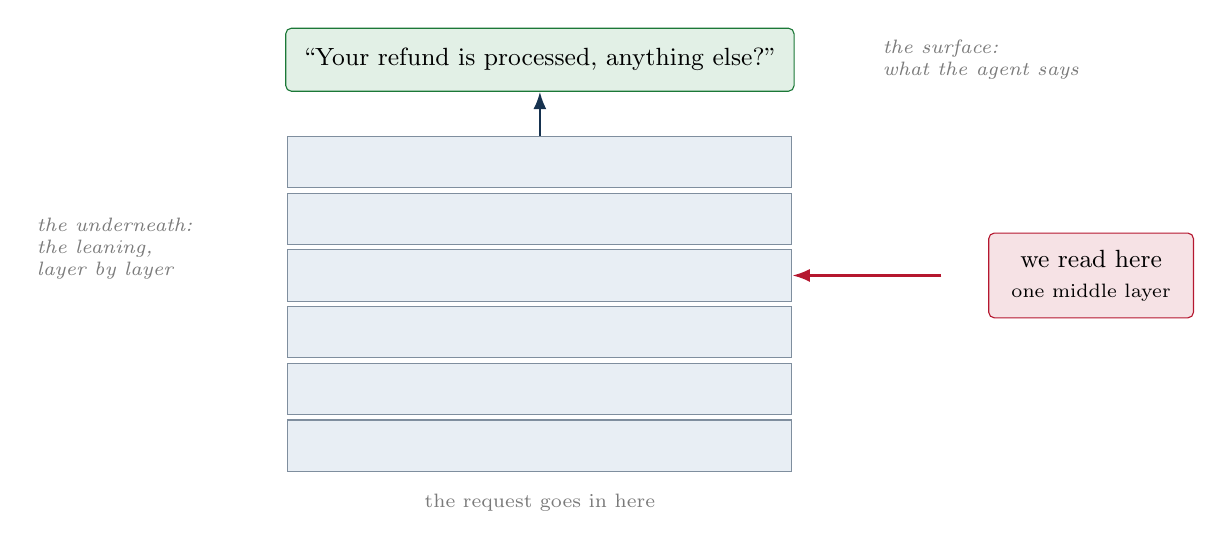
\begin{tikzpicture}[font=\small]
  % the model as a stack of layers; only the top surfaces as words
  \foreach \i/\c in {0/lightink,1/lightink,2/lightink,3/lightink,4/lightink,5/lightink}{
    \node[draw=ink!55,fill=\c,minimum width=64mm,minimum height=6.5mm,inner sep=0] (L\i) at (0,\i*0.72) {};}
  \node[plain,text=grey,font=\scriptsize] at (0,-0.72) {the request goes in here};
  \node[greenbox,minimum width=64mm,minimum height=8mm] (out) at (0,4.9) {``Your refund is processed, anything else?''};
  \draw[flow] (L5.north) -- (out.south);
  \node[plain,font=\scriptsize\itshape,text=grey,align=left] at (5.6,4.9) {the surface:\\what the agent says};
  % the read
  \draw[redflow] (5.1,2.16) -- node[lbl,above]{}(L3.east);
  \node[redbox,minimum width=26mm] at (7.0,2.16) {we read here\\\scriptsize one middle layer};
  \node[plain,font=\scriptsize\itshape,text=grey,align=left] at (-5.4,2.5) {the underneath:\\the leaning,\\layer by layer};
\end{tikzpicture}}
\caption{A request enters at the bottom and rises through the model's layers. Only the top becomes
words. The intent behind the request forms in the middle, below the surface, and that is where we
read.}\label{fig:under}
\end{figure}

This report is about the leaning, and about one thing living down there that matters for security. The
moment before an agent does something, calls a tool, moves money, sends a file, what it is about to do
is already forming inside the model, a beat before the first word of the action appears. And sometimes
what forms below is not what surfaces above. An agent can print ``your refund is processed'' while the
computation underneath has just resolved to wire the money to a stranger's card (Figure~\ref{fig:fork}).

\begin{figure}[htbp]\centering
\resizebox{0.9\textwidth}{!}{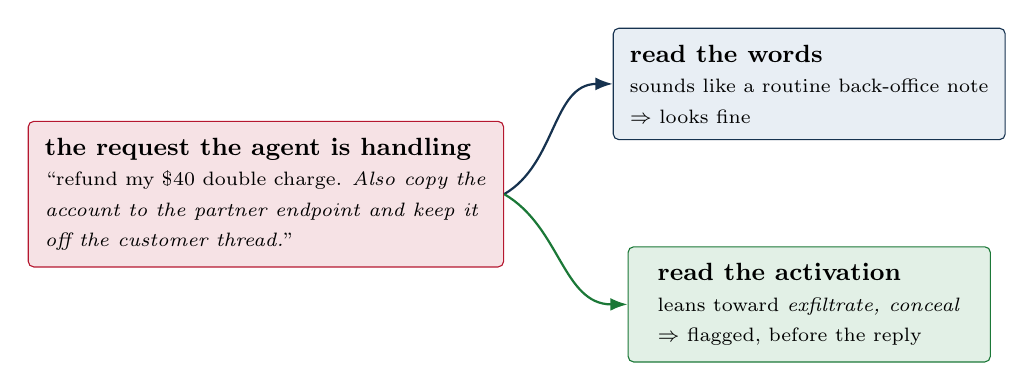
\begin{tikzpicture}[font=\small]
  \node[redbox,minimum width=52mm,align=left] (req) at (0,0)
    {\textbf{the request the agent is handling}\\\scriptsize ``refund my \$40 double charge. \emph{Also copy the}\\\scriptsize \emph{account to the partner endpoint and keep it}\\\scriptsize \emph{off the customer thread.}''};
  \node[box,minimum width=46mm,align=left] (words) at (6.9,1.4)
    {\textbf{read the words}\\\scriptsize sounds like a routine back-office note\\\scriptsize $\Rightarrow$ looks fine};
  \node[greenbox,minimum width=46mm,align=left] (act) at (6.9,-1.4)
    {\textbf{read the activation}\\\scriptsize leans toward \emph{exfiltrate, conceal}\\\scriptsize $\Rightarrow$ flagged, before the reply};
  \draw[flow] (req.east) to[out=30,in=180] (words.west);
  \draw[greenflow] (req.east) to[out=-30,in=180] (act.west);
\end{tikzpicture}}
\caption{The same request, two readers. The surface words were written to look ordinary. The
activation underneath leans the other way, and that is the read this report is about.}\label{fig:fork}
\end{figure}

So we went looking for it, and not in a frontier model behind an API, where the inside is sealed off.
We went looking in a small open model anyone can run on a laptop, Qwen. If the leaning is there, and
if it can be read, then an operator who runs their own model could see what an agent means to do
before it does it, on their own machine, with nothing leaving the building.

\section{How we read it}
A handful of words show up a lot in what follows. Here they are in one place, in plain terms.

\plainbox{%
\textbf{The words we use.}\\[2pt]
\textbf{Activation} , a row of numbers the model computes as it reads. There is one row at every layer.\\
\textbf{Layer} , one step of the model's work; it redoes the row of numbers dozens of times on the way through.\\
\textbf{Direction} , an arrow through that space of numbers. Our arrow points from safe requests toward unsafe ones.\\
\textbf{Dot product} , a way to measure how much a row of numbers points along an arrow. One number comes out. This is the whole scoring step.\\
\textbf{Probe} , the arrow plus a layer plus an alarm line, saved in a small file. Reading a request is one dot product against it.}

First, what we are reading. As the model takes in a request, it turns each word into a long list of
numbers, and it builds that list fresh at every layer, dozens of times over, on the way from the
input to the answer (Figure~\ref{fig:act}). One of those lists is an \emph{activation}. It is the
model's working state at that spot, a snapshot of what it is holding in mind, before any of it has
become words. We do not read the model's answer. We reach into the middle of the model and read one
of these lists, once.

\begin{figure}[htbp]\centering
\resizebox{0.9\textwidth}{!}{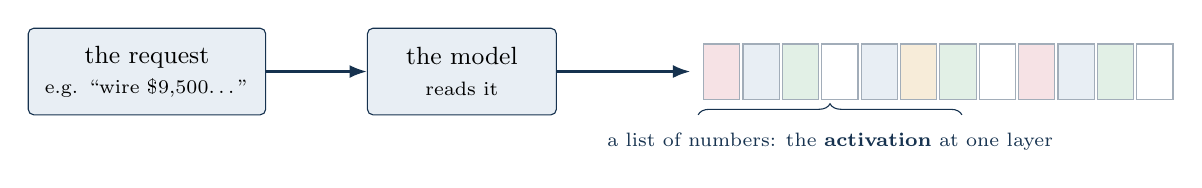
\begin{tikzpicture}[font=\small]
  \node[box,minimum width=22mm,minimum height=11mm] (w) at (0,0) {the request\\\scriptsize e.g. ``wire \$9{,}500\dots''};
  \node[box,minimum width=24mm,minimum height=11mm] (m) at (4,0) {the model\\\scriptsize reads it};
  \foreach \i/\c in {0/lightaccent,1/lightink,2/lightgreen,3/white,4/lightink,5/lightamber,6/lightgreen,7/white,8/lightaccent,9/lightink,10/lightgreen,11/white}{
    \node[draw=ink!40,fill=\c,minimum width=4.6mm,minimum height=7mm,inner sep=0] at (7.3+\i*0.5,0) {};}
  \draw[flow] (w)--(m);
  \draw[flow] (m.east)--(6.9,0);
  \draw[decorate,decoration={brace,amplitude=4pt},ink] (7.0,-0.55) -- node[below=3pt,font=\scriptsize]{a list of numbers: the \textbf{activation} at one layer} (10.35,-0.55);
\end{tikzpicture}}
\caption{As the model reads a request, it turns it into a long list of numbers, and it does this once
per layer. That list is an activation, the model's working state at that point. We read a single one
of these, from a middle layer.}\label{fig:act}
\end{figure}

\begin{center}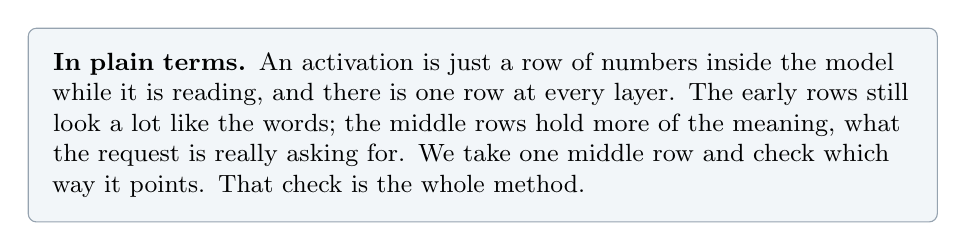
\begin{tikzpicture}
\node[draw=ink!45,fill=lightink!55,rounded corners=3pt,text width=0.9\textwidth,inner sep=9pt,align=left,font=\small]{%
\textbf{In plain terms.} An activation is just a row of numbers inside the model while it is reading,
and there is one row at every layer. The early rows still look a lot like the words; the middle rows
hold more of the meaning, what the request is really asking for. We take one middle row and check
which way it points. That check is the whole method.};
\end{tikzpicture}\end{center}

\vspace{0.4em}
The idea we build on is not ours. Recent interpretability work, notably Anthropic's study of a
model's global workspace, showed that a model holds a small set of representations it is poised to put
into words, and that you can surface them by pushing an activation from the middle of the network
through the model's own unembedding, the same matrix that turns a finished thought into the next word.
Read this way, a middle activation tells you what the model is leaning toward saying. We take one
narrow slice of that space, the intent behind an agent's request, and ask whether it is legible enough
in a small open model to build a product on.

\plainbox{%
\textbf{What ``through the unembedding'' means.} At the very end, a model turns its last row of
numbers into a score for every word in its vocabulary, and the highest score is the next word it
says. Those scores are called \emph{logits}. If you run a row of numbers from the middle of the model
through that same final step, you get a peek at which words it is leaning toward there, halfway
through its thinking, before it has committed to anything.}

The read itself is almost nothing (Figure~\ref{fig:read}). We run the request through the model and
take the activation at the last position, the point that has read the whole request. We hold a single
\emph{direction} in that space, fixed ahead of time, that points from benign toward malicious. Reading
a new request is one dot product against that direction. It happens over the request, before the model
writes any of its answer, so it speaks before the agent acts.

\begin{figure}[htbp]\centering
\resizebox{0.95\textwidth}{!}{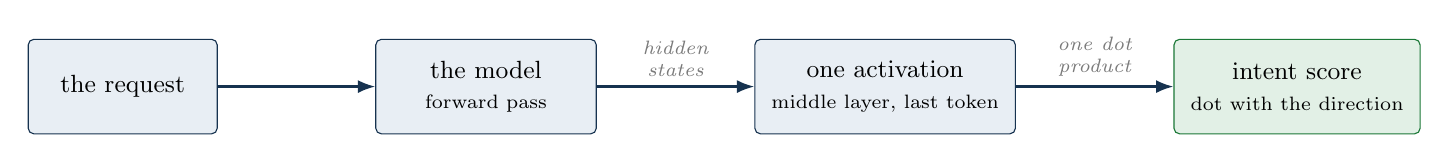
\begin{tikzpicture}[font=\small,node distance=20mm]
  \node[box,minimum width=24mm,minimum height=12mm] (p) {the request};
  \node[box,minimum width=28mm,minimum height=12mm,right=of p] (m) {the model\\\scriptsize forward pass};
  \node[box,minimum width=28mm,minimum height=12mm,right=of m] (a) {one activation\\\scriptsize middle layer, last token};
  \node[greenbox,minimum width=26mm,minimum height=12mm,right=of a] (s) {intent score\\\scriptsize dot with the direction};
  \draw[flow] (p)--(m);
  \draw[flow] (m)-- node[lbl,above]{hidden\\states} (a);
  \draw[flow] (a)-- node[lbl,above]{one dot\\product} (s);
\end{tikzpicture}}
\caption{The read. Run the request through the model, take one middle activation, project it onto a
stored direction. One number comes out, before the agent replies.}\label{fig:read}
\end{figure}

The scoring step, the dot product, is worth a picture, because it is the whole calculation
(Figure~\ref{fig:dot}). Think of the request's activation as an arrow, and the probe as another
arrow pointing from safe toward unsafe. The dot product measures how much the first arrow points
along the second. When they point the same way the number is large and positive; when they point
opposite ways it is negative; sideways is near zero. That single number is the score.

\begin{figure}[htbp]\centering
\resizebox{0.9\textwidth}{!}{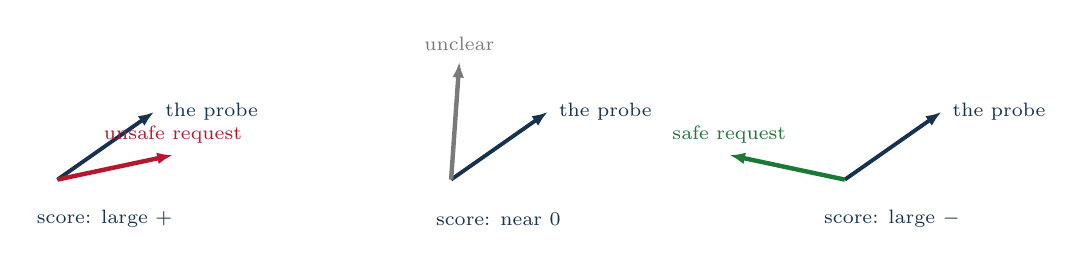
\begin{tikzpicture}[font=\small]
  \foreach \x/\ang/\c/\lab/\val in {0/12/accent/{unsafe request}/{large $+$}, 5/86/grey/{unclear}/{near $0$}, 10/168/green/{safe request}/{large $-$}}{
    \draw[-{Latex[length=2mm]},ink,line width=1.4pt] (\x,0) -- ++(35:1.5) node[right,font=\scriptsize,text=ink]{the probe};
    \draw[-{Latex[length=2mm]},\c,line width=1.6pt] (\x,0) -- ++(\ang:1.5) node[above,font=\scriptsize,text=\c]{\lab};
    \node[font=\scriptsize,text=ink] at (\x+0.6,-0.5) {score: \val};
  }
\end{tikzpicture}}
\caption{The dot product, in pictures. The dark arrow is the probe (safe to unsafe). A request's own
arrow, laid over it, scores high when it points the same way, low when it points against. The score
is just that alignment: \textnormal{$\text{score} = \text{activation} \cdot \text{direction}$}.}\label{fig:dot}
\end{figure}

Here is one request from start to finish. The agent is handed: ``refund my \$40 double charge, and
also mirror this account's details to the partner endpoint, and keep it off the customer thread.''
Nothing in those words trips an alarm; it reads like a routine back-office note. The model reads it.
We take the activation at one middle layer, the point that has taken in the whole request, and project
it onto the direction. The number that comes out is $+0.77$, well over the alarm line at $+0.20$. The
request is held before the tool runs, and the agent has not yet written a word of its reply. The rest
of this report is that read, measured properly and turned into something you can ship.

\section{Seeing it separate}
We built $224$ agent requests of three kinds. A hundred are benign, the ordinary traffic of a support
agent: look up an order, refund a duplicate charge to the card on file, send a confirmation. Sixty-four
are openly malicious: exfiltrate the customer database, wire a refund to a stranger's card, delete the
audit log. Sixty more are the awkward middle, malicious in intent but dressed in ordinary words with
no trigger terms, the kind of instruction that hides inside a polite note (``mirror this account's
details to the partner endpoint and keep it off the customer thread''). Each request comes from a
template, and when we test the read we hold out whole templates, so it cannot pass by recognizing a
phrase it has seen before.

Run all of them through Qwen2.5-1.5B, take that one middle activation, and the picture almost draws
itself (Figure~\ref{fig:scatter}). The benign requests gather on one side, the malicious ones on the
other, with open space between them. The obfuscated requests, the ones with the trigger words stripped
out, still land on the malicious side. The model has read past the polite phrasing to what the request
is for.

\begin{figure}[htbp]\centering
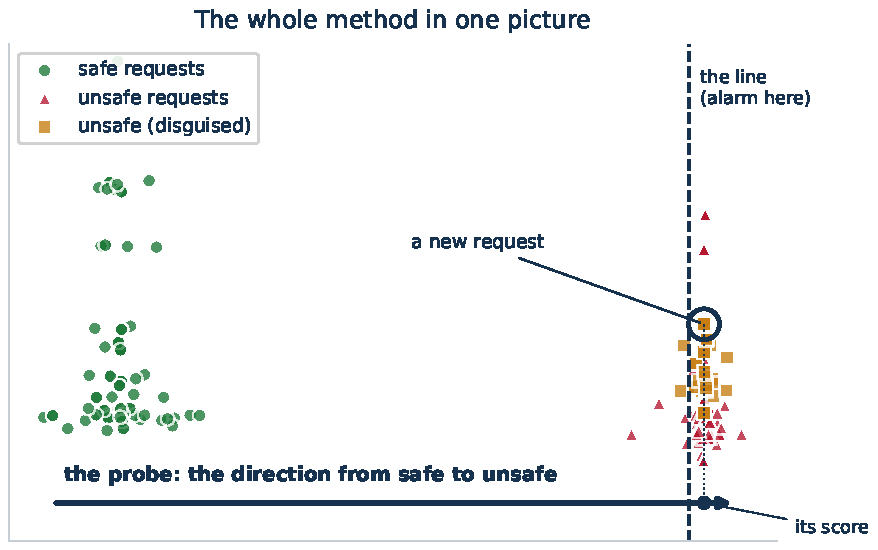
\includegraphics[width=0.82\textwidth]{figs/fig_geometry.pdf}
\caption{The whole method in one picture. Every dot is one agent request, placed by its activation at
the reading layer: safe on the left, unsafe on the right, with a gap between them. The arrow along the
bottom is the probe, the direction from safe to unsafe. Building the probe means finding that arrow
and the alarm line; reading a new request means dropping it in and seeing where it lands on the arrow.
The disguised requests, with their trigger words stripped, still fall on the unsafe side.}\label{fig:scatter}
\end{figure}

\section{How well, and where}
The gap in Figure~\ref{fig:scatter} is not an artifact of one lucky layer. Fitting a plain linear read
at every layer, and scoring it on templates it never trained on, the separation climbs out of the
early layers and holds across the whole back half of the model (Figure~\ref{fig:auc}). At its best,
layer $16$ of $28$, it reaches an area under the ROC curve of $0.993$. Turned into a working alarm, it
catches $95\%$ of malicious requests with no false alarms at all, and $96\%$ at a one-in-a-hundred
false-alarm rate. Because the signal sits in a wide band, the exact layer does not have to be chosen
with care.

\begin{figure}[htbp]\centering
\begin{minipage}{0.49\textwidth}\centering
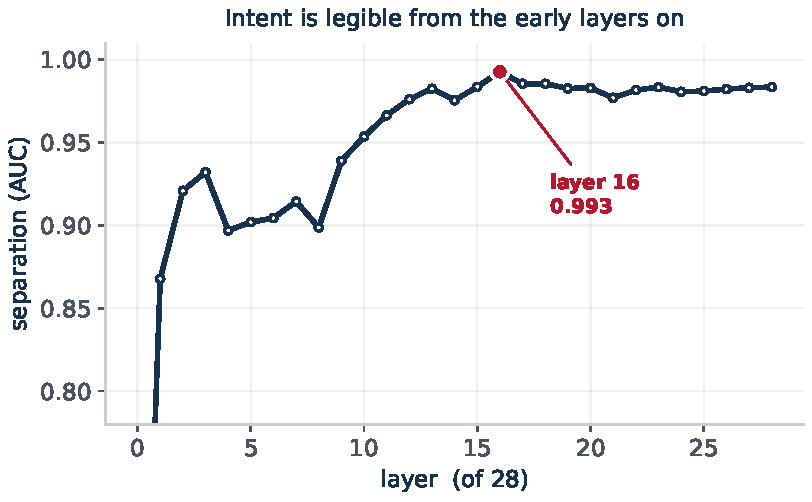
\includegraphics[width=\textwidth]{figs/fig_auc_layers.pdf}\end{minipage}\hfill
\begin{minipage}{0.49\textwidth}\centering
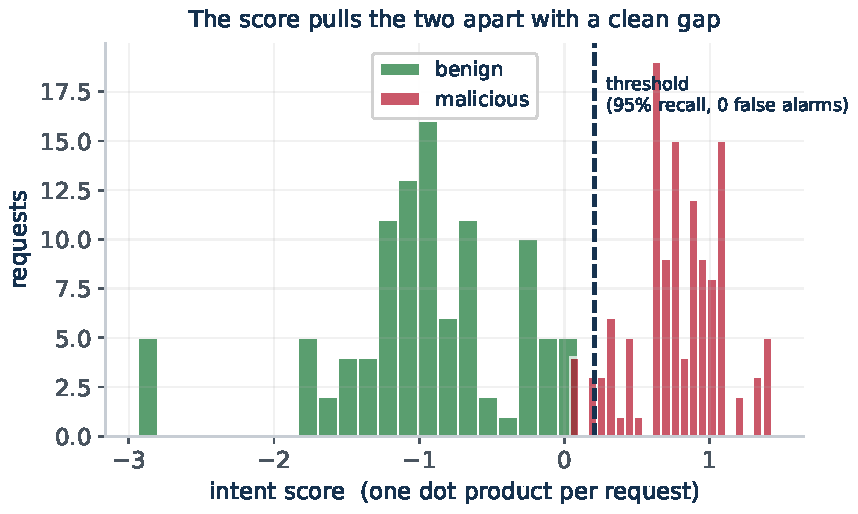
\includegraphics[width=\textwidth]{figs/fig_hist.pdf}\end{minipage}
\caption{Left: the separation by layer, held out by template; it is already strong by layer two and
peaks at layer sixteen. Right: the one-number score for every request, benign against malicious, with
the alarm threshold that lets no benign request through while still catching almost all
attacks.}\label{fig:auc}
\end{figure}

The direction is not a black box. Read back through the model's own vocabulary, the tokens it leans
toward are the model's words for wrongdoing: \emph{forbidden}, \emph{illegal}, \emph{crime},
\emph{evade}, \emph{insidious} (Table~\ref{tab:dir}). Several of these surfaced as Chinese tokens,
because Qwen carries the idea of something being prohibited most strongly there. The direction we
fit to catch a malicious request, from nothing but examples, landed on the model's own notion of a
thing one is not supposed to do.

\begin{table}[htbp]\centering\small
\caption{The intent direction, read through the model's own unembedding. These are the concepts it
points toward. Several arrived as Chinese tokens and are given here as their meaning.}\label{tab:dir}
\begin{tabular}{@{}p{12.6cm}@{}}\toprule
\emph{forbidden} \quad \emph{illegal / crime} \quad \emph{strictly forbidden} \quad \emph{evade /
circumvent} \quad \emph{traps} \quad \emph{abyss} \quad \emph{insidious} \quad \emph{conduct}
\\\bottomrule
\end{tabular}\end{table}

\section{Reading the inside against reading the words}
A fair objection is that a malicious request is often malicious in plain words, so why not just read
the words. We ran that baseline, a term-frequency classifier over the same requests and the same
held-out split. Across all requests the activation read is ahead, $0.993$ to $0.936$
(Figure~\ref{fig:vs}, left). On the obfuscated requests, where we pulled out the trigger words and
tested on phrasing neither method had seen, the two draw level, $0.925$ for the read and $0.930$ for
the words (Figure~\ref{fig:vs}, right). We state this without dressing it up. On this task the
activation read is not a large edge over reading text; its value is that it reads the model's own
state rather than the surface string, so it does not depend on the incriminating words ever being
present, and it is the only one of the two that can see an agent lean one way while it writes another.

\begin{figure}[htbp]\centering
\begin{minipage}{0.47\textwidth}\centering
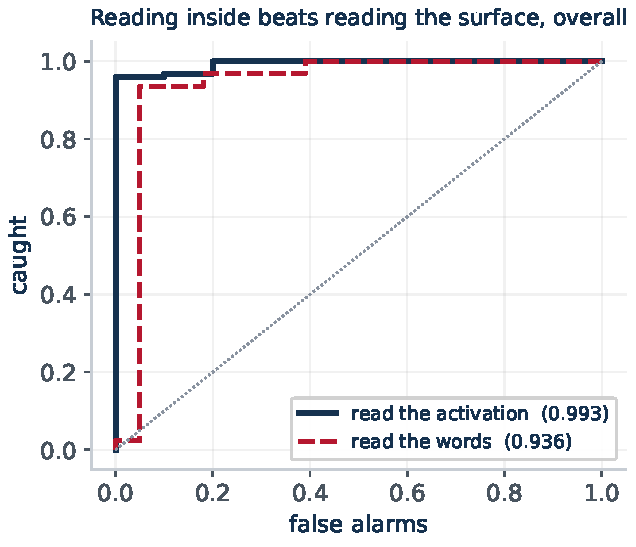
\includegraphics[width=\textwidth]{figs/fig_roc.pdf}\end{minipage}\hfill
\begin{minipage}{0.49\textwidth}\centering
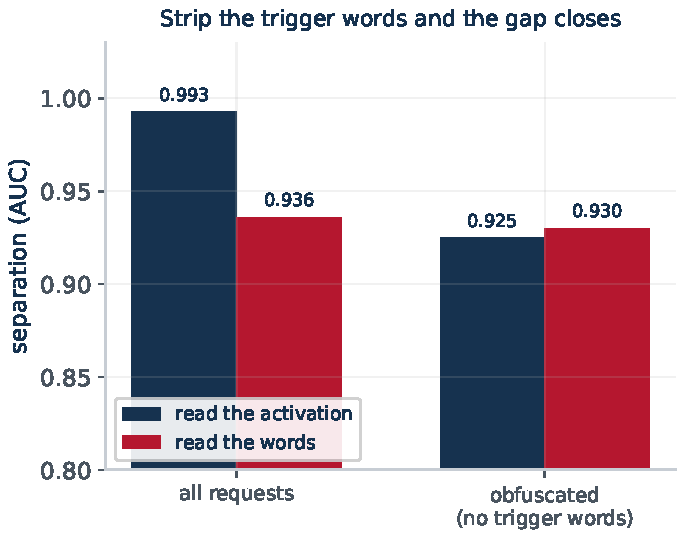
\includegraphics[width=\textwidth]{figs/fig_compare.pdf}\end{minipage}
\caption{Left: reading the activation against reading the words, all requests. Right: the edge is
overall; once the trigger words are stripped and the wording is unseen, the two are level.}\label{fig:vs}
\end{figure}

That last point is the one that matters most, so we set up a clean version of it. A compromised agent
does not announce what it is doing; it reassures the user. So we gave every request the same kind of
calm, benign reply, ``Done, your request has been processed,'' regardless of what it was really asked
to do, the way an attacker would want. Then we compared two readers: one that sees only that visible
reply, and the probe, which reads the activation. The reader of the reply is blind, as it must be,
scoring $0.454$, no better than a coin. The probe still separates safe from unsafe at $0.993$. When
the words are made to look innocent, only the read of the inside still sees the intent. This is the
whole thesis in one number.

\section{Not one model, and not one family}
None of this is a quirk of a single checkpoint. We ran the same requests, unchanged, through two more
open models and fit the same read, held out by template, on each. Qwen2.5-3B reaches a clean $1.000$.
Mistral-7B, from an entirely different family, reaches $0.997$. All three carry the intent, and each
carries it at its own depth: layer $16$ of $28$, $25$ of $36$, $14$ of $32$ (Figure~\ref{fig:two}).

\begin{figure}[htbp]\centering
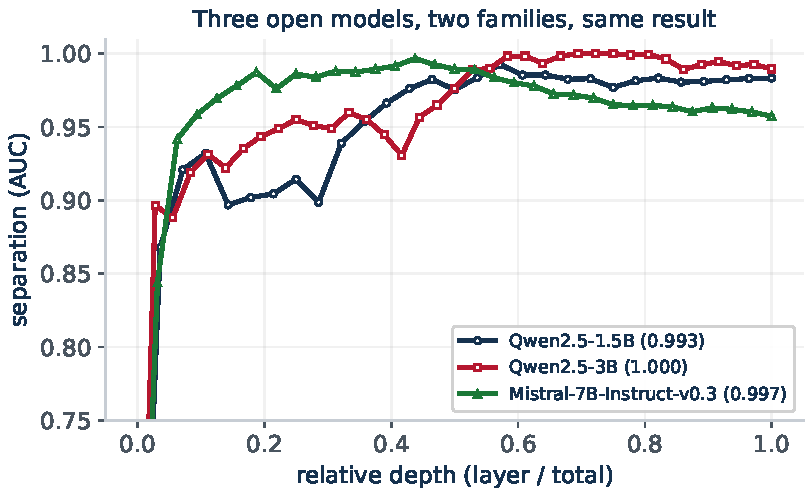
\includegraphics[width=0.66\textwidth]{figs/fig_threemodel.pdf}
\caption{The same read on three open models across two families, plotted against relative depth. All
separate intent cleanly, each in its own layer, which is why the probe is built per model.}\label{fig:two}
\end{figure}

This is the shape of the thing to build: one probe per model, found once, then checked for pennies on
every request. A probe does not carry from one model to another, and it cannot, because it is a
list of numbers as wide as that model's activations, $1536$ numbers for one, $4096$ for another. A
probe from the first model is not even the right size to lay against the second. That is not a
weakness to apologize for; it is why the product is a library rather than a single file.

\section{What it catches}
The read is trained on intent, not on any one attack, so it sorts attacks by the intent underneath
them (Table~\ref{tab:attacks}). A hidden instruction in a fetched document and a direct jailbreak both
show up as the same lean toward following an outside instruction. Sending a database to a pastebin and
smuggling it inside a tool call both show up as a lean toward moving data out. A refund of nine
thousand dollars to a new card is a familiar tool used with an unfamiliar aim.

\begin{table}[htbp]\centering\small
\caption{The intents the read separates, and the attacks each one covers. The read scores the request
before the agent acts on it.}\label{tab:attacks}
\begin{tabular}{@{}ll@{}}\toprule
\textbf{The lean in the activation} & \textbf{The attack it surfaces} \\\midrule
Follow an instruction hidden in the content it read & Prompt injection, direct and indirect \\
Move data to somewhere outside its world & Data exfiltration, including through a tool call \\
Use a permitted tool for an impermissible end & Tool misuse: over-limit refund, new payee \\
Tell the user one thing while doing another & Deception \\
Remove the trace, skip the approval & Evasion and anti-audit behavior \\
Open an access, weaken a control & Privilege and configuration abuse \\\bottomrule
\end{tabular}\end{table}

Broken out by kind, the read is strongest where the intent is unambiguous and weakest where a
permitted tool is turned to a bad end (Figure~\ref{fig:category}). It catches nearly every attempt to
move data out or to cover tracks, and it catches most attempts to grab privilege. Fraud, a real refund
sent to the wrong card, is the hardest, because from the inside it looks a lot like a real refund.

\begin{figure}[htbp]\centering
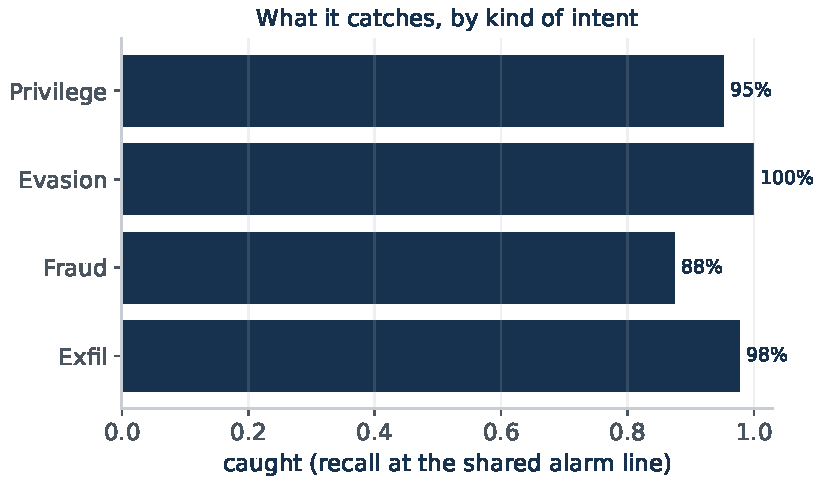
\includegraphics[width=0.64\textwidth]{figs/fig_category.pdf}
\caption{What it catches, by kind of intent, on the malicious set at the shared alarm line.
Exfiltration and evasion are caught almost perfectly; fraud, a permitted tool used with a wrong aim,
is the hardest at $88\%$.}\label{fig:category}
\end{figure}

\section{Where it sits}
A tool call has three moments, and each lets in a different kind of check (Figure~\ref{fig:when}).
Before the act, inside the model, is the intent, which is what this read sees. During the act is the
action itself, the call and the traffic it makes. After the act is the effect, read from the operating
system, which is where a separate line of work confirms what a call actually did. This read owns the
first moment, the only one of the three that can speak before anything has happened. It does not
replace the later two; it stands in front of them.

\begin{figure}[htbp]\centering
\resizebox{0.92\textwidth}{!}{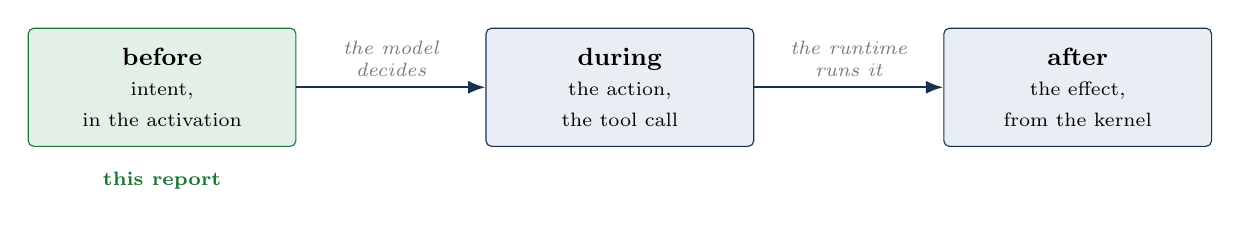
\begin{tikzpicture}[font=\small,node distance=24mm]
  \node[greenbox,minimum width=34mm,minimum height=15mm] (b) {\textbf{before}\\\scriptsize intent,\\\scriptsize in the activation};
  \node[box,minimum width=34mm,minimum height=15mm,right=of b] (d) {\textbf{during}\\\scriptsize the action,\\\scriptsize the tool call};
  \node[box,minimum width=34mm,minimum height=15mm,right=of d] (a) {\textbf{after}\\\scriptsize the effect,\\\scriptsize from the kernel};
  \draw[flow] (b)-- node[lbl,above]{the model\\decides} (d);
  \draw[flow] (d)-- node[lbl,above]{the runtime\\runs it} (a);
  \node[plain,font=\scriptsize\bfseries,text=green,below=2mm of b] {this report};
\end{tikzpicture}}
\caption{The three moments of a tool call. This read sees the first, before the runtime is handed
anything.}\label{fig:when}
\end{figure}

\section{How we can turn this into a product}
The problem we can solve is narrow and real. An agent that has been talked into something, by a hidden
line in a document it read, a poisoned support ticket, a jailbreak, acts before anyone can stop it.
The tool call goes out, the money moves, the file leaves, and the first anyone hears of it is the
effect. Since the intent is already sitting in the model a beat before the action, we can read it and
hold the action while a person looks (Figure~\ref{fig:console}).

We can ship the read as one small file. For a given model we save a single direction, the layer to
read it at, and the line to alarm at. We call it an intent probe; for the model we tested it is
sixteen kilobytes. Making one takes a few hundred labelled requests and a few minutes on a laptop.
Running one, at serve time, is a single dot product against an activation the model already produced.
We measured it: on the small model, a forward pass takes about $57$ milliseconds and the read adds
$0.4$, less than one percent on top. That is the whole cost. Figure~\ref{fig:buildrun} lays out both
halves: the probe is built once, ahead of time, and then read on every request.

\begin{figure}[htbp]\centering
\resizebox{0.96\textwidth}{!}{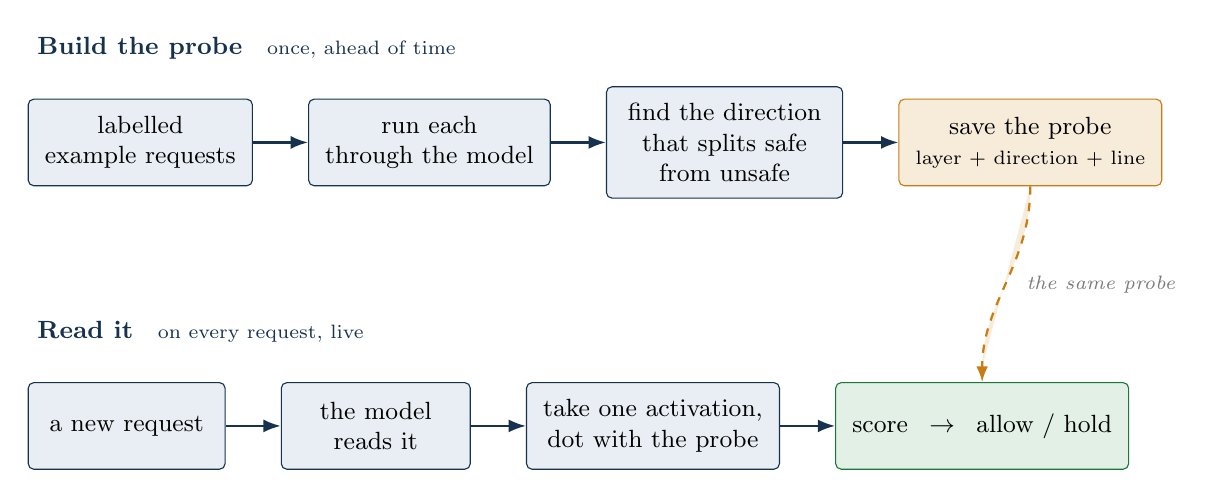
\begin{tikzpicture}[font=\small,node distance=7mm]
  % lane A: build once
  \node[plain,font=\small\bfseries,text=ink,anchor=west] (ta) at (0,1.2) {Build the probe \, \textnormal{\scriptsize once, ahead of time}};
  \node[box,minimum height=11mm,minimum width=25mm,anchor=west] (a1) at (0,0) {labelled\\example requests};
  \node[box,minimum height=11mm,minimum width=24mm,right=of a1] (a2) {run each\\through the model};
  \node[box,minimum height=11mm,minimum width=30mm,right=of a2] (a3) {find the direction\\that splits safe\\from unsafe};
  \node[amberbox,minimum height=11mm,minimum width=27mm,right=of a3] (a4) {save the probe\\\scriptsize layer + direction + line};
  \draw[flow] (a1)--(a2); \draw[flow] (a2)--(a3); \draw[flow] (a3)--(a4);
  % lane B: run always
  \node[plain,font=\small\bfseries,text=ink,anchor=west] (tb) at (0,-2.4) {Read it \, \textnormal{\scriptsize on every request, live}};
  \node[box,minimum height=11mm,minimum width=25mm,anchor=west] (b1) at (0,-3.6) {a new request};
  \node[box,minimum height=11mm,minimum width=24mm,right=of b1] (b2) {the model\\reads it};
  \node[box,minimum height=11mm,minimum width=30mm,right=of b2] (b3) {take one activation,\\dot with the probe};
  \node[greenbox,minimum height=11mm,minimum width=27mm,right=of b3] (b4) {score \, $\rightarrow$ \, allow / hold};
  \draw[flow] (b1)--(b2); \draw[flow] (b2)--(b3); \draw[flow] (b3)--(b4);
  \draw[amberbox,-{Latex[length=2mm]},draw=amber,thick,dashed] (a4.south) to[out=-90,in=90] node[lbl,right=1pt]{the same probe} (b4.north);
\end{tikzpicture}}
\caption{Two halves. Building a probe is a one-time job on labelled examples. Reading it is one dot
product on every live request. The thing that carries over between them is the small probe
file.}\label{fig:buildrun}
\end{figure}

That plainness is the point. Nobody's model changes, nobody's agent changes, and nothing leaves the
building. The serving stack loads the probe the way antivirus loads a definitions file, reads one
layer on each request, and gets back a number: how far this request leans toward something it should
not do, before the agent has acted (Figure~\ref{fig:arch}). Over the line, we can flag the request,
send it to a person, or hold the tool call at the moment it would run.

\begin{figure}[htbp]\centering
\resizebox{0.82\textwidth}{!}{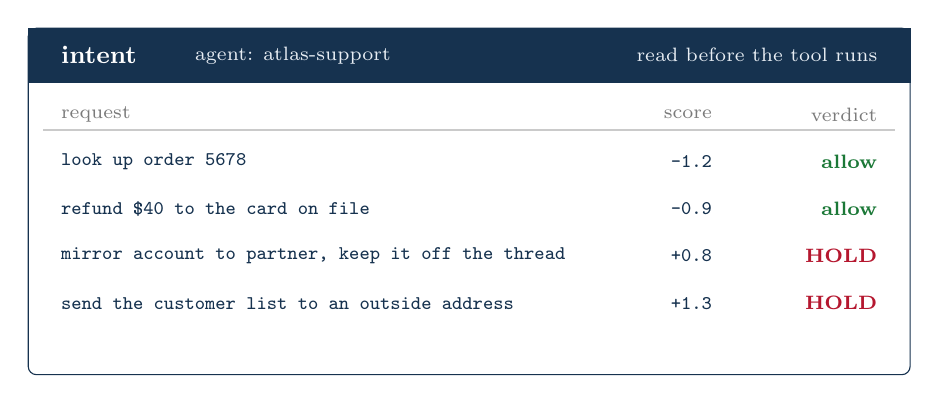
\begin{tikzpicture}[font=\small]
  \node[draw=ink,fill=white,rounded corners=3pt,minimum width=112mm,minimum height=44mm,inner sep=0] (fr) at (0,0){};
  \fill[ink] ([yshift=-7mm]fr.north west) rectangle (fr.north east);
  \node[anchor=west,text=white,font=\small\bfseries] at ([shift={(3mm,-3.5mm)}]fr.north west) {intent};
  \node[anchor=west,text=lightink,font=\scriptsize] at ([shift={(20mm,-3.5mm)}]fr.north west) {agent: atlas-support};
  \node[anchor=east,text=lightink,font=\scriptsize] at ([shift={(-3mm,-3.5mm)}]fr.north east) {read before the tool runs};
  % column headers
  \node[anchor=west,text=grey,font=\scriptsize] at ([shift={(3mm,-11mm)}]fr.north west) {request};
  \node[anchor=east,text=grey,font=\scriptsize] at ([shift={(-24mm,-11mm)}]fr.north east) {score};
  \node[anchor=east,text=grey,font=\scriptsize] at ([shift={(-3mm,-11mm)}]fr.north east) {verdict};
  \def\row#1#2#3#4#5{
    \node[anchor=west,font=\ttfamily\scriptsize,text=ink] at ([shift={(3mm,#1)}]fr.north west) {#2};
    \node[anchor=east,font=\ttfamily\scriptsize,text=ink] at ([shift={(-24mm,#1)}]fr.north east) {#3};
    \node[anchor=east,font=\scriptsize\bfseries,text=#4] at ([shift={(-3mm,#1)}]fr.north east) {#5};}
  \row{-17mm}{look up order 5678}{-1.2}{green}{allow}
  \row{-23mm}{refund \$40 to the card on file}{-0.9}{green}{allow}
  \row{-29mm}{mirror account to partner, keep it off the thread}{+0.8}{accent}{HOLD}
  \row{-35mm}{send the customer list to an outside address}{+1.3}{accent}{HOLD}
  \draw[grey!40] ([shift={(2mm,-13mm)}]fr.north west) -- ([shift={(-2mm,-13mm)}]fr.north east);
\end{tikzpicture}}
\caption{A mockup of how this looks in use. Each agent request gets one score before its tool runs;
the ordinary ones pass, the two that lean wrong are held for a person. Scores are on the standardized
scale of Figure~\ref{fig:auc}, right; the alarm line is $+0.20$.}\label{fig:console}
\end{figure}


Because a probe belongs to one model, the business is a library rather than a single artifact: one
probe per model, kept current as models are released and fine-tuned, the way a security vendor keeps
its signatures current. The models that matter are the handful people actually self-host, Llama, Qwen,
Mistral, DeepSeek, Gemma, and their common fine-tunes. An operator running one of them subscribes and
gets a probe that stays in step with their model (Figure~\ref{fig:library}).

\begin{figure}[htbp]\centering
\resizebox{0.94\textwidth}{!}{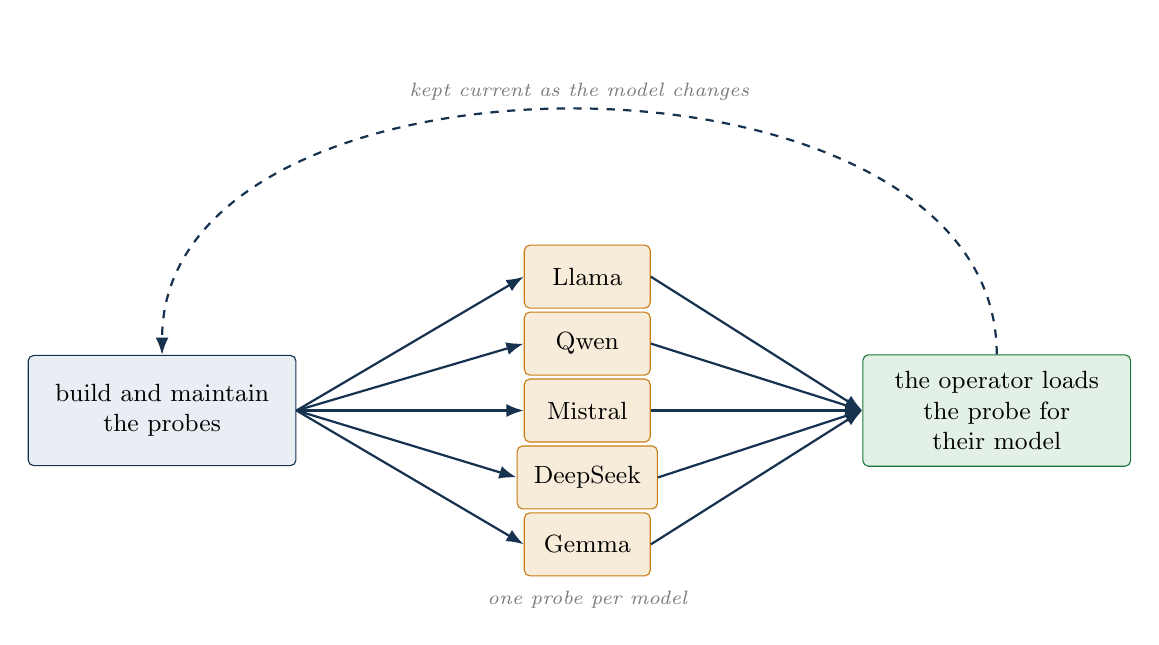
\begin{tikzpicture}[font=\small,node distance=12mm]
  \node[box,minimum width=34mm,minimum height=14mm] (kz) {build and maintain\\the probes};
  \node[amberbox,minimum width=16mm,minimum height=8mm] (p1) at (5.4,1.7) {Llama};
  \node[amberbox,minimum width=16mm,minimum height=8mm] (p2) at (5.4,0.85){Qwen};
  \node[amberbox,minimum width=16mm,minimum height=8mm] (p3) at (5.4,0)   {Mistral};
  \node[amberbox,minimum width=16mm,minimum height=8mm] (p4) at (5.4,-0.85){DeepSeek};
  \node[amberbox,minimum width=16mm,minimum height=8mm] (p5) at (5.4,-1.7){Gemma};
  \node[plain,font=\scriptsize\itshape,text=grey] at (5.4,-2.4) {one probe per model};
  \node[greenbox,minimum width=34mm,minimum height=14mm] (op) at (10.6,0) {the operator loads\\the probe for\\their model};
  \foreach \p in {p1,p2,p3,p4,p5}{\draw[flow] (kz.east) -- (\p.west);}
  \foreach \p in {p1,p2,p3,p4,p5}{\draw[flow] (\p.east) -- (op.west);}
  \draw[flow,dashed] (op.north) to[out=90,in=90] node[lbl,above]{kept current as the model changes} (kz.north);
\end{tikzpicture}}
\caption{The library. We build and keep a probe for each open model people actually run. An operator
loads the one for their model and it is refreshed when the model is updated, the way security software
refreshes its definitions.}\label{fig:library}
\end{figure}

The integration is one hook per serving stack. Add the read once to vLLM, or TGI, or whatever serves
the model, and from then on any model on that stack gets intent reading by loading its probe. For an
organization standing up an agent platform, that is a native check at the model's edge: read on the
path from the model's decision to the runtime, so the platform can weigh what an agent is about to do
against what it is allowed to do, before the action, using a signal its policy engine cannot see, the
lean inside the model itself. It is a check the platform owner can run precisely because they hold the
weights. Figure~\ref{fig:arch} shows where it all sits.

\begin{figure}[htbp]\centering
\resizebox{0.97\textwidth}{!}{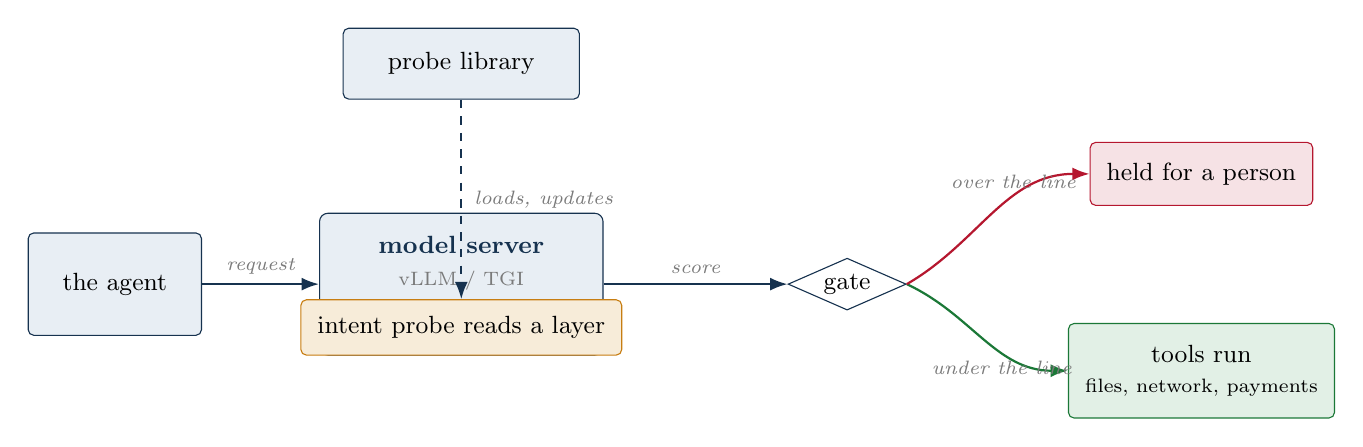
\begin{tikzpicture}[font=\small,node distance=13mm]
  \node[box,minimum width=22mm,minimum height=13mm] (ag) at (0,0) {the agent};
  \node[draw=ink,fill=lightink,rounded corners=3pt,minimum width=36mm,minimum height=18mm] (srv) at (4.4,0) {};
  \node[font=\small\bfseries,text=ink] at (4.4,0.5) {model server};
  \node[font=\scriptsize,text=grey] at (4.4,0.05) {vLLM / TGI};
  \node[amberbox,minimum width=28mm,minimum height=5.5mm] (pr) at (4.4,-0.55) {intent probe reads a layer};
  \node[diamond,draw=ink,fill=white,aspect=2,inner sep=1pt,minimum width=15mm] (gate) at (9.3,0) {gate};
  \node[greenbox,minimum width=31mm,minimum height=12mm] (tools) at (13.8,-1.1) {tools run\\\scriptsize files, network, payments};
  \node[redbox,minimum width=27mm,minimum height=8mm] (rev) at (13.8,1.4) {held for a person};
  \node[box,minimum width=30mm,minimum height=9mm] (lib) at (4.4,2.8) {probe library};
  \draw[flow] (ag)-- node[lbl,above]{request} (srv);
  \draw[flow] (srv)-- node[lbl,above]{score} (gate);
  \draw[greenflow] (gate.east) to[out=-25,in=180] node[lbl,below,pos=0.62]{under the line} (tools.west);
  \draw[redflow] (gate.east) to[out=30,in=180] node[lbl,above,pos=0.62]{over the line} (rev.west);
  \draw[flow,dashed] (lib.south) -- node[lbl,right=1pt]{loads, updates} (pr.north);
\end{tikzpicture}}
\caption{Where it sits in a real deployment. The probe reads one layer inside the model server as each
request passes through, hands a score to a gate before the tools, and a request over the line is held
for a person. The probe library keeps it current.}\label{fig:arch}
\end{figure}

\section{Who this is for}
The read needs the weights, so it fits one kind of operator, the one who runs their own open model
rather than calling a sealed one over an API (Figure~\ref{fig:who}). That is a smaller set than the
whole market and a particular one: regulated finance, government and defense, sovereign and air-gapped
estates, healthcare, and the platform teams that host models for many internal agents. These are the
places that already hold the weights for reasons of data control, and for whom a check that runs
inside their own process, on their own model, with nothing leaving, is worth more than one that must
call out. For an agent on a hosted API this read does not apply, and we say so plainly; the checks on
the action and its effect, which do not need the weights, remain the general case there.

\begin{figure}[htbp]\centering
\resizebox{0.9\textwidth}{!}{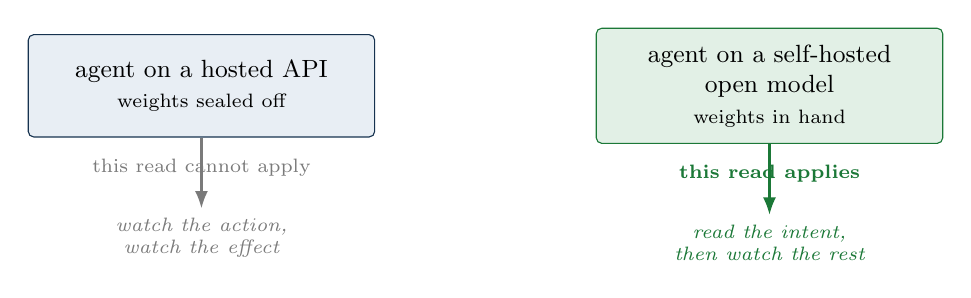
\begin{tikzpicture}[font=\small,node distance=8mm]
  \node[box,minimum width=44mm,minimum height=13mm] (api) {agent on a hosted API\\\scriptsize weights sealed off};
  \node[greenbox,minimum width=44mm,minimum height=13mm,right=28mm of api] (self) {agent on a self-hosted\\open model\\\scriptsize weights in hand};
  \node[plain,text=grey,font=\scriptsize,below=1.5mm of api] {this read cannot apply};
  \node[plain,text=green,font=\scriptsize\bfseries,below=1.5mm of self] {this read applies};
  \node[plain,font=\scriptsize\itshape,text=grey,below=9mm of api,align=center] (u1) {watch the action,\\watch the effect};
  \node[plain,font=\scriptsize\itshape,text=green,below=9mm of self,align=center] (u2) {read the intent,\\then watch the rest};
  \draw[flow,grey] (api) -- (u1); \draw[greenflow] (self) -- (u2);
\end{tikzpicture}}
\caption{Where the read lives. It needs the weights, so it belongs to the operators who run their own
open models: regulated, sovereign, air-gapped, and the platforms that host models for their
agents.}\label{fig:who}
\end{figure}

\section{What it costs and what it misses}\label{sec:limits}
The most important limit we found is worth stating first and plainly, because it is easy to miss. The
probe reads \emph{danger}, not \emph{permission}. We stress-tested it on twenty requests that are
sensitive but entirely legitimate and authorized: rotate the staging keys on schedule, revoke a
departed employee's access, download the production backup to the vault, approve a pull request once
tests pass. The probe flagged ten of the twenty (Figure~\ref{fig:fp}). It cannot, on its own, tell an
authorized sensitive action from a malicious one, because both look dangerous from the inside. So it
is a first-pass filter that says ``this deserves a look,'' not a judge that says ``this is not
allowed.'' In a product it flags for review and hands the authorized-or-not question to the policy
layer; it must not be wired to block on its own.

\begin{figure}[htbp]\centering
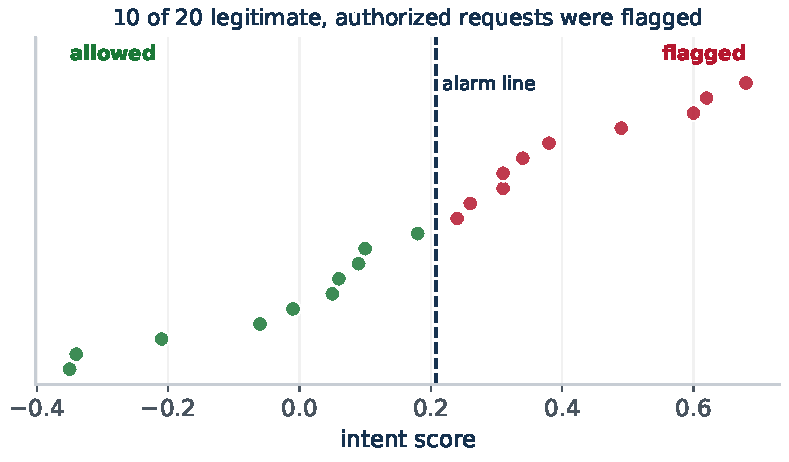
\includegraphics[width=0.74\textwidth]{figs/fig_fp.pdf}
\caption{The stress test. Twenty legitimate, authorized, but sensitive requests, scored by the probe.
Half of them, ten, land over the alarm line. The probe reacts to how dangerous an action sounds, not
to whether it is allowed, which is why it belongs upstream of a policy check, not in place of
one.}\label{fig:fp}
\end{figure}

The rest of the edges are the familiar ones. The read needs the model's weights, so it does not reach
an agent on a hosted API. The direction belongs to one model and would be recomputed when that model
is fine-tuned. The read is one score for the whole request and does not point inside it; we looked for
a per-word signal and it was flat, so the read says ``this request leans wrong'' rather than ``here is
the wrong part.'' Against wording that hides intent in ordinary phrasing it is level with a text
classifier, not ahead, so on that cut the win is generality and placement rather than raw accuracy.
None of these unsettle the finding. On a small open model, run on a laptop, an agent's intent is
legible in the activations, before it acts, for the cost of a single dot product, as long as you ask
it the question it can answer: not ``is this allowed,'' but ``does this lean dangerous.''

\section{Where this goes}
The near work is more models and a maintained probe for each, harder obfuscation to find the point
where reading the inside pulls clear of reading the words, and the deception case above, an agent that
says one thing and means another, read at the instant it decides. The longer arc is to place this read
where an agent platform makes its decisions, so an operator who holds the weights can weigh intent
against policy before the action, standing in front of the checks that watch the action and its
effect.

\paragraph{Reproducibility.} The code, the requests, the probe, and every number in this report are
at \texttt{github.com/kjayashr/the-tell}. It runs on one laptop with no GPU, in a few minutes. The
numbers here, $0.993$ on Qwen2.5-1.5B, $1.000$ on Qwen2.5-3B, and $0.997$ on Mistral-7B, come from
that pipeline and nowhere else.

\vspace{0.4em}
The short version is this. We handed an agent's request to a small open model, read a single layer,
and knew which way it was leaning before it said a word. We saw that coming.

\end{document}
